
%% Drawing and using free body diagrams: Why it may be better not to decompose forces
%% Ivica Aviani, Natasa Erceg, and Vanes Mesic
%% Phys. Rev. ST Phys. Educ. Res. 10, 020137--Published 2015
%% DOI: 10.1103/PhysRevSTPER.11.020137


%% Free Body Diagrams, 020137 pp12
%%--------------------------------------------------
\element{FBD}{
\begin{question}{FBD-Q01}
    A block is resting on a horizontal surface.
    Which of the following diagrams correctly shows the forces acting on the block?
    \begin{multicols}{2}
    \begin{choices}
        \AMCboxDimensions{down=-1.5cm}
        \wrongchoice{
            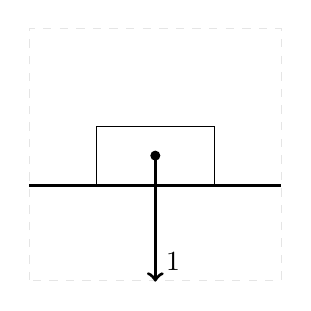
\begin{tikzpicture}[scale=0.8]
                \draw[dashed,white!90!black] (-2,-1.5) rectangle (2,2.5);
                \draw[very thick] (-2,0) -- (2,0);
                \node[draw,minimum width=1.5cm,minimum height=0.75cm,anchor=south] (B) at (0,0) {};
                \draw[fill] (B.center) circle (2pt);
                \draw[very thick,->] (B.center) -- ++(270:2) node[anchor=south west] {1};
            \end{tikzpicture}
        }
        \wrongchoice{
            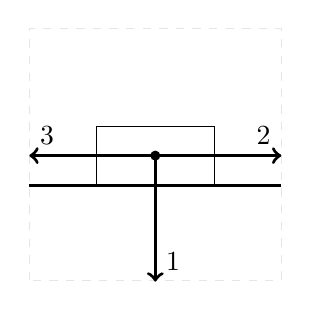
\begin{tikzpicture}[scale=0.8]
                \draw[dashed,white!90!black] (-2,-1.5) rectangle (2,2.5);
                \draw[very thick] (-2,0) -- (2,0);
                \node[draw,minimum width=1.5cm,minimum height=0.75cm,anchor=south] (B) at (0,0) {};
                \draw[fill] (B.center) circle (2pt);
                \draw[very thick,->] (B.center) -- ++(270:2) node[anchor=south west] {1};
                \draw[very thick,->] (B.center) -- ++(0:2) node[anchor=south east] {2};
                \draw[very thick,->] (B.center) -- ++(180:2) node[anchor=south west] {3};
            \end{tikzpicture}
        }
        \correctchoice{
            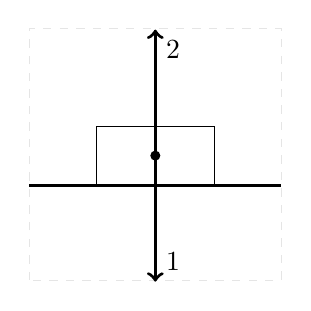
\begin{tikzpicture}[scale=0.8]
                \draw[dashed,white!90!black] (-2,-1.5) rectangle (2,2.5);
                \draw[very thick] (-2,0) -- (2,0);
                \node[draw,minimum width=1.5cm,minimum height=0.75cm,anchor=south] (B) at (0,0) {};
                \draw[fill] (B.center) circle (2pt);
                \draw[very thick,->] (B.center) -- ++(270:2) node[anchor=south west] {1};
                \draw[very thick,->] (B.center) -- ++(90:2) node[anchor=north west] {2};
            \end{tikzpicture}
        }
        \wrongchoice{
            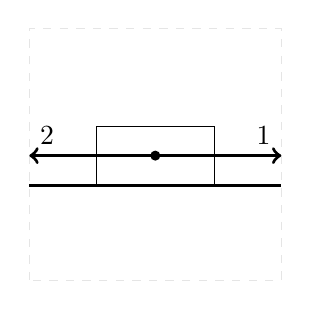
\begin{tikzpicture}[scale=0.8]
                \draw[dashed,white!90!black] (-2,-1.5) rectangle (2,2.5);
                \draw[very thick] (-2,0) -- (2,0);
                \node[draw,minimum width=1.5cm,minimum height=0.75cm,anchor=south] (B) at (0,0) {};
                \draw[fill] (B.center) circle (2pt);
                \draw[very thick,->] (B.center) -- ++(180:2) node[anchor=south west] {2};
                \draw[very thick,->] (B.center) -- ++(0:2) node[anchor=south east] {1};
            \end{tikzpicture}
        }
        \wrongchoice{
            \begin{tikzpicture}[scale=0.8]
                \draw[dashed,white!90!black] (-2,-1.5) rectangle (2,2.5);
                \draw[very thick] (-2,0) -- (2,0);
                \node[draw,minimum width=1.5cm,minimum height=0.75cm,anchor=south] (B) at (0,0) {};
                \draw[fill] (B.center) circle (2pt);
                \draw[very thick,->] (B.center) -- ++(90:2) node[anchor=south west] {1};
            \end{tikzpicture}
        }
    \end{choices}
    \end{multicols}
\end{question}
}

\element{FBD}{
\begin{question}{FBD-Q02}
    The pulling force $F$ is acting on a block, but the block is still at rest.
    Which of the following diagrams correctly shows the forces acting on the block?
    \begin{multicols}{2}
    \begin{choices}
        \AMCboxDimensions{down=-1.5cm}
        \wrongchoice{
            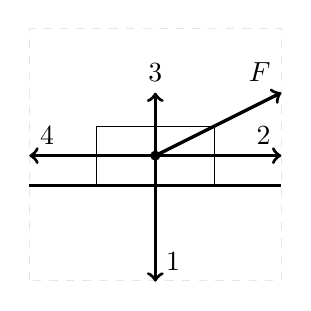
\begin{tikzpicture}[scale=0.8]
                \draw[dashed,white!90!black] (-2,-1.5) rectangle (2,2.5);
                \draw[very thick] (-2,0) -- (2,0);
                \node[draw,minimum width=1.5cm,minimum height=0.75cm,anchor=south] (B) at (0,0) {};
                \draw[fill] (B.center) circle (2pt);
                \draw[very thick,->] (B.center) -- ++(270:2) node[anchor=south west] {1};
                \draw[very thick,->] (B.center) -- ++(0:2) node[anchor=south east] {2};
                \draw[very thick,->] (B.center) -- ++(90:1) node[anchor=south] {3};
                \draw[very thick,->] (B.center) -- ++(180:2) node[anchor=south west] {4};
                \draw[very thick,->] (B.center) -- ++(2,1) node[anchor=south east] {$F$};
            \end{tikzpicture}
        }
        \wrongchoice{
            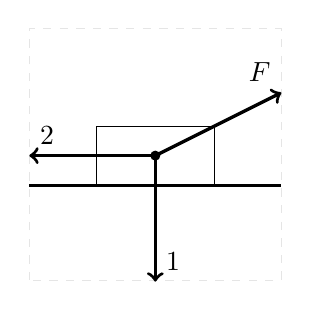
\begin{tikzpicture}[scale=0.8]
                \draw[dashed,white!90!black] (-2,-1.5) rectangle (2,2.5);
                \draw[very thick] (-2,0) -- (2,0);
                \node[draw,minimum width=1.5cm,minimum height=0.75cm,anchor=south] (B) at (0,0) {};
                \draw[fill] (B.center) circle (2pt);
                \draw[very thick,->] (B.center) -- ++(270:2) node[anchor=south west] {1};
                \draw[very thick,->] (B.center) -- ++(180:2) node[anchor=south west] {2};
                \draw[very thick,->] (B.center) -- ++(2,1) node[anchor=south east] {$F$};
            \end{tikzpicture}
        }
        \wrongchoice{
            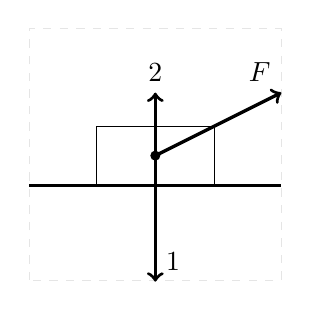
\begin{tikzpicture}[scale=0.8]
                \draw[dashed,white!90!black] (-2,-1.5) rectangle (2,2.5);
                \draw[very thick] (-2,0) -- (2,0);
                \node[draw,minimum width=1.5cm,minimum height=0.75cm,anchor=south] (B) at (0,0) {};
                \draw[fill] (B.center) circle (2pt);
                \draw[very thick,->] (B.center) -- ++(270:2) node[anchor=south west] {1};
                \draw[very thick,->] (B.center) -- ++(90:1) node[anchor=south] {2};
                \draw[very thick,->] (B.center) -- ++(2,1) node[anchor=south east] {$F$};
            \end{tikzpicture}
        }
        \wrongchoice{
            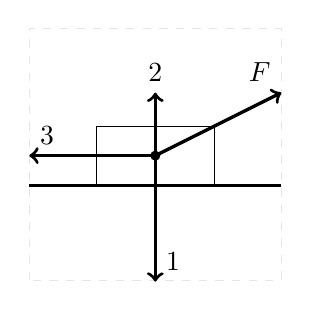
\begin{tikzpicture}[scale=0.8]
                \draw[dashed,white!90!black] (-2,-1.5) rectangle (2,2.5);
                \draw[very thick] (-2,0) -- (2,0);
                \node[draw,minimum width=1.5cm,minimum height=0.75cm,anchor=south] (B) at (0,0) {};
                \draw[fill] (B.center) circle (2pt);
                \draw[very thick,->] (B.center) -- ++(270:2) node[anchor=south west] {1};
                \draw[very thick,->] (B.center) -- ++(90:1) node[anchor=south] {2};
                \draw[very thick,->] (B.center) -- ++(180:2) node[anchor=south west] {3};
                \draw[very thick,->] (B.center) -- ++(2,1) node[anchor=south east] {$F$};
            \end{tikzpicture}
        }
        \correctchoice{
            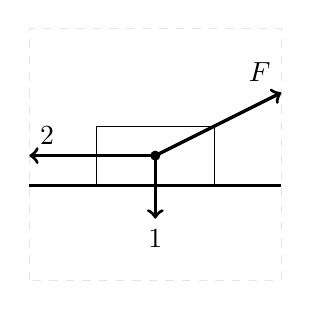
\begin{tikzpicture}[scale=0.8]
                \draw[dashed,white!90!black] (-2,-1.5) rectangle (2,2.5);
                \draw[very thick] (-2,0) -- (2,0);
                \node[draw,minimum width=1.5cm,minimum height=0.75cm,anchor=south] (B) at (0,0) {};
                \draw[fill] (B.center) circle (2pt);
                \draw[very thick,->] (B.center) -- ++(270:1) node[anchor=north] {1};
                \draw[very thick,->] (B.center) -- ++(180:2) node[anchor=south west] {2};
                \draw[very thick,->] (B.center) -- ++(2,1) node[anchor=south east] {$F$};
            \end{tikzpicture}
        }
    \end{choices}
    \end{multicols}
\end{question}
}

\element{FBD}{
\begin{question}{FBD-Q03}
    A block is sliding along a horizontal surface at constant speed.
    Which of the following diagrams correctly shows the forces acting on the block?
    \begin{multicols}{2}
    \begin{choices}
        \AMCboxDimensions{down=-1.5cm}
        \wrongchoice{
            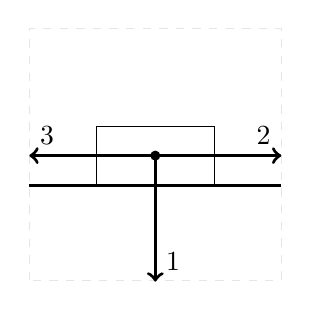
\begin{tikzpicture}[scale=0.8]
                \draw[dashed,white!90!black] (-2,-1.5) rectangle (2,2.5);
                \draw[very thick] (-2,0) -- (2,0);
                \node[draw,minimum width=1.5cm,minimum height=0.75cm,anchor=south] (B) at (0,0) {};
                \draw[fill] (B.center) circle (2pt);
                \draw[very thick,->] (B.center) -- ++(270:2) node[anchor=south west] {1};
                \draw[very thick,->] (B.center) -- ++(0:2) node[anchor=south east] {2};
                \draw[very thick,->] (B.center) -- ++(180:2) node[anchor=south west] {3};
            \end{tikzpicture}
        }
        \wrongchoice{
            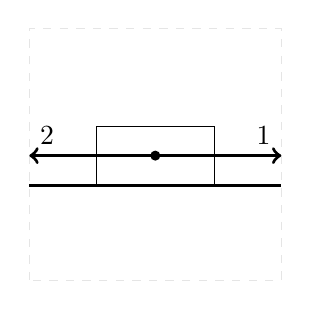
\begin{tikzpicture}[scale=0.8]
                \draw[dashed,white!90!black] (-2,-1.5) rectangle (2,2.5);
                \draw[very thick] (-2,0) -- (2,0);
                \node[draw,minimum width=1.5cm,minimum height=0.75cm,anchor=south] (B) at (0,0) {};
                \draw[fill] (B.center) circle (2pt);
                \draw[very thick,->] (B.center) -- ++(0:2) node[anchor=south east] {1};
                \draw[very thick,->] (B.center) -- ++(180:2) node[anchor=south west] {2};
            \end{tikzpicture}
        }
        \wrongchoice{
            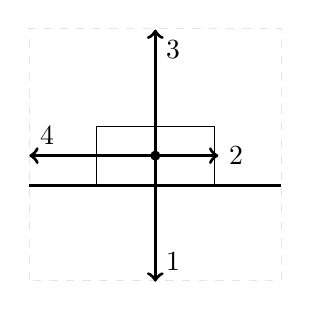
\begin{tikzpicture}[scale=0.8]
                \draw[dashed,white!90!black] (-2,-1.5) rectangle (2,2.5);
                \draw[very thick] (-2,0) -- (2,0);
                \node[draw,minimum width=1.5cm,minimum height=0.75cm,anchor=south] (B) at (0,0) {};
                \draw[fill] (B.center) circle (2pt);
                \draw[very thick,->] (B.center) -- ++(270:2) node[anchor=south west] {1};
                \draw[very thick,->] (B.center) -- ++(0:1) node[anchor=west] {2};
                \draw[very thick,->] (B.center) -- ++(90:2) node[anchor=north west] {3};
                \draw[very thick,->] (B.center) -- ++(180:2) node[anchor=south west] {4};
            \end{tikzpicture}
        }
        \wrongchoice{
            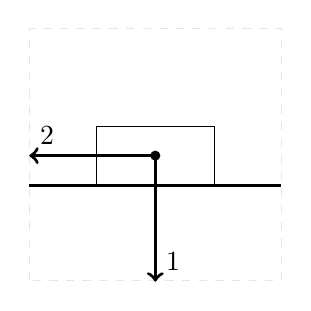
\begin{tikzpicture}[scale=0.8]
                \draw[dashed,white!90!black] (-2,-1.5) rectangle (2,2.5);
                \draw[very thick] (-2,0) -- (2,0);
                \node[draw,minimum width=1.5cm,minimum height=0.75cm,anchor=south] (B) at (0,0) {};
                \draw[fill] (B.center) circle (2pt);
                \draw[very thick,->] (B.center) -- ++(270:2) node[anchor=south west] {1};
                \draw[very thick,->] (B.center) -- ++(180:2) node[anchor=south west] {2};
            \end{tikzpicture}
        }
        \correctchoice{
            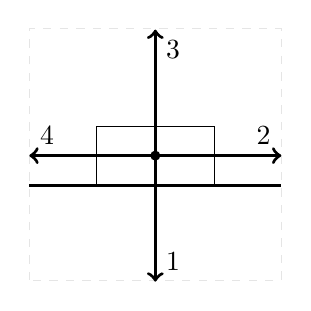
\begin{tikzpicture}[scale=0.8]
                \draw[dashed,white!90!black] (-2,-1.5) rectangle (2,2.5);
                \draw[very thick] (-2,0) -- (2,0);
                \node[draw,minimum width=1.5cm,minimum height=0.75cm,anchor=south] (B) at (0,0) {};
                \draw[fill] (B.center) circle (2pt);
                \draw[very thick,->] (B.center) -- ++(270:2) node[anchor=south west] {1};
                \draw[very thick,->] (B.center) -- ++(0:2) node[anchor=south east] {2};
                \draw[very thick,->] (B.center) -- ++(90:2) node[anchor=north west] {3};
                \draw[very thick,->] (B.center) -- ++(180:2) node[anchor=south west] {4};
            \end{tikzpicture}
        }
    \end{choices}
    \end{multicols}
\end{question}
}

\element{FBD}{
\begin{question}{FBD-Q04}
    A block is accelerating along a horizontal surface.
    Which of the following diagrams correctly shows the forces acting on the block?
    \begin{multicols}{2}
    \begin{choices}
        \AMCboxDimensions{down=-1.5cm}
        %% NOTE: we cannot ignore friction, see A and B
        \correctchoice{
            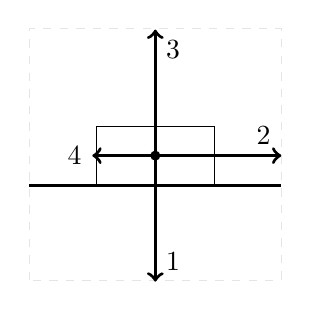
\begin{tikzpicture}[scale=0.8]
                \draw[dashed,white!90!black] (-2,-1.5) rectangle (2,2.5);
                \draw[very thick] (-2,0) -- (2,0);
                \node[draw,minimum width=1.5cm,minimum height=0.75cm,anchor=south] (B) at (0,0) {};
                \draw[fill] (B.center) circle (2pt);
                \draw[very thick,->] (B.center) -- ++(270:2) node[anchor=south west] {1};
                \draw[very thick,->] (B.center) -- ++(0:2) node[anchor=south east] {2};
                \draw[very thick,->] (B.center) -- ++(90:2) node[anchor=north west] {3};
                \draw[very thick,->] (B.center) -- ++(180:1) node[anchor=east] {4};
            \end{tikzpicture}
        }
        \wrongchoice{
            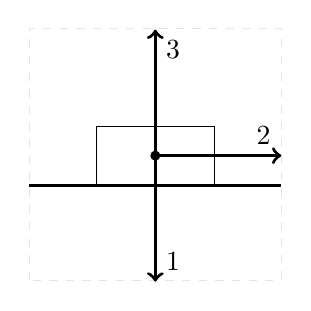
\begin{tikzpicture}[scale=0.8]
                \draw[dashed,white!90!black] (-2,-1.5) rectangle (2,2.5);
                \draw[very thick] (-2,0) -- (2,0);
                \node[draw,minimum width=1.5cm,minimum height=0.75cm,anchor=south] (B) at (0,0) {};
                \draw[fill] (B.center) circle (2pt);
                \draw[very thick,->] (B.center) -- ++(270:2) node[anchor=south west] {1};
                \draw[very thick,->] (B.center) -- ++(0:2) node[anchor=south east] {2};
                \draw[very thick,->] (B.center) -- ++(90:2) node[anchor=north west] {3};
            \end{tikzpicture}
        }
        \wrongchoice{
            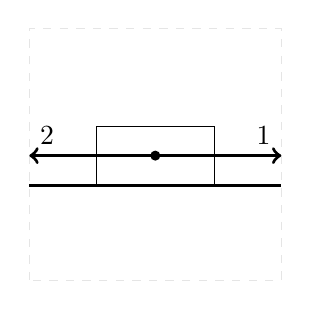
\begin{tikzpicture}[scale=0.8]
                \draw[dashed,white!90!black] (-2,-1.5) rectangle (2,2.5);
                \draw[very thick] (-2,0) -- (2,0);
                \node[draw,minimum width=1.5cm,minimum height=0.75cm,anchor=south] (B) at (0,0) {};
                \draw[fill] (B.center) circle (2pt);
                \draw[very thick,->] (B.center) -- ++(0:2) node[anchor=south east] {1};
                \draw[very thick,->] (B.center) -- ++(180:2) node[anchor=south west] {2};
            \end{tikzpicture}
        }
        \wrongchoice{
            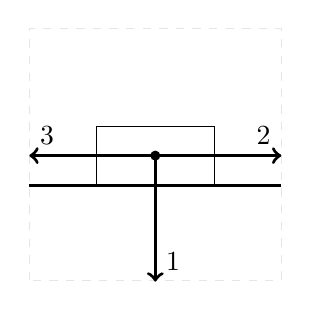
\begin{tikzpicture}[scale=0.8]
                \draw[dashed,white!90!black] (-2,-1.5) rectangle (2,2.5);
                \draw[very thick] (-2,0) -- (2,0);
                \node[draw,minimum width=1.5cm,minimum height=0.75cm,anchor=south] (B) at (0,0) {};
                \draw[fill] (B.center) circle (2pt);
                \draw[very thick,->] (B.center) -- ++(270:2) node[anchor=south west] {1};
                \draw[very thick,->] (B.center) -- ++(0:2) node[anchor=south east] {2};
                \draw[very thick,->] (B.center) -- ++(180:2) node[anchor=south west] {3};
            \end{tikzpicture}
        }
        \wrongchoice{
            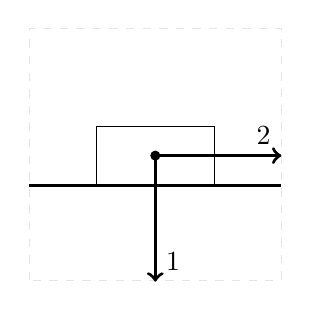
\begin{tikzpicture}[scale=0.8]
                \draw[dashed,white!90!black] (-2,-1.5) rectangle (2,2.5);
                \draw[very thick] (-2,0) -- (2,0);
                \node[draw,minimum width=1.5cm,minimum height=0.75cm,anchor=south] (B) at (0,0) {};
                \draw[fill] (B.center) circle (2pt);
                \draw[very thick,->] (B.center) -- ++(270:2) node[anchor=south west] {1};
                \draw[very thick,->] (B.center) -- ++(0:2) node[anchor=south east] {2};
            \end{tikzpicture}
        }
    \end{choices}
    \end{multicols}
\end{question}
}

\element{FBD}{
\begin{question}{FBD-Q05}
    A block is resting on an inclined plane.
    Which of the following diagrams correctly shows the forces on the block?
    \begin{multicols}{2}
    \begin{choices}
        \AMCboxDimensions{down=-1.5cm}
        \wrongchoice{
            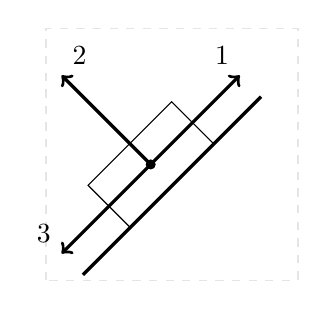
\begin{tikzpicture}[scale=0.8]
                \draw[dashed,white!90!black] (-2,-1.5) rectangle (2,2.5);
                \node[draw,minimum width=1.5cm,minimum height=0.75cm,anchor=south,rotate=45] (B) at (0,0) {};
                \draw[very thick,rotate=45] (-2,0) -- (2,0);
                \draw[fill] (B.center) circle (2pt);
                \draw[very thick,->] (B.center) -- ++(45:2) node[anchor=south east] {1};
                \draw[very thick,->] (B.center) -- ++(135:2) node[anchor=south west] {2};
                \draw[very thick,->] (B.center) -- ++(225:2) node[anchor=south east] {3};
            \end{tikzpicture}
        }
        \correctchoice{
            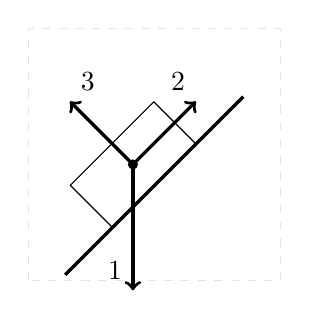
\begin{tikzpicture}[scale=0.8]
                \draw[dashed,white!90!black] (-2,-1.5) rectangle (2,2.5);
                \node[draw,minimum width=1.5cm,minimum height=0.75cm,anchor=south,rotate=45] (B) at (0,0) {};
                \draw[very thick,rotate=45] (-2,0) -- (2,0);
                \draw[fill] (B.center) circle (2pt);
                \draw[very thick,->] (B.center) -- ++(270:2) node[anchor=south east] {1};
                \draw[very thick,->] (B.center) -- ++(45:1.414) node[anchor=south east] {2};
                \draw[very thick,->] (B.center) -- ++(135:1.414) node[anchor=south west] {3};
            \end{tikzpicture}
        }
        \wrongchoice{
            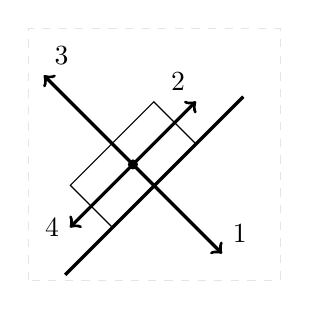
\begin{tikzpicture}[scale=0.8]
                \draw[dashed,white!90!black] (-2,-1.5) rectangle (2,2.5);
                \node[draw,minimum width=1.5cm,minimum height=0.75cm,anchor=south,rotate=45] (B) at (0,0) {};
                \draw[very thick,rotate=45] (-2,0) -- (2,0);
                \draw[fill] (B.center) circle (2pt);
                \draw[very thick,->] (B.center) -- ++(315:2) node[anchor=south west] {1};
                \draw[very thick,->] (B.center) -- ++(45:1.414) node[anchor=south east] {2};
                \draw[very thick,->] (B.center) -- ++(135:2) node[anchor=south west] {3};
                \draw[very thick,->] (B.center) -- ++(225:1.414) node[anchor=east] {4};
            \end{tikzpicture}
        }
        \wrongchoice{
            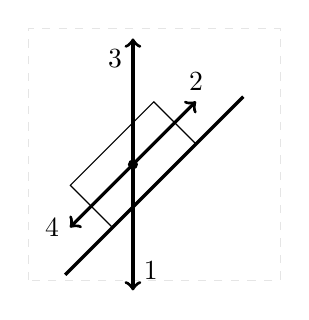
\begin{tikzpicture}[scale=0.8]
                \draw[dashed,white!90!black] (-2,-1.5) rectangle (2,2.5);
                \node[draw,minimum width=1.5cm,minimum height=0.75cm,anchor=south,rotate=45] (B) at (0,0) {};
                \draw[very thick,rotate=45] (-2,0) -- (2,0);
                \draw[fill] (B.center) circle (2pt);
                \draw[very thick,->] (B.center) -- ++(270:2) node[anchor=south west] {1};
                \draw[very thick,->] (B.center) -- ++(45:1.414) node[anchor=south] {2};
                \draw[very thick,->] (B.center) -- ++(90:2) node[anchor=north east] {3};
                \draw[very thick,->] (B.center) -- ++(225:1.414) node[anchor=east] {4};
            \end{tikzpicture}
        }
        \wrongchoice{
            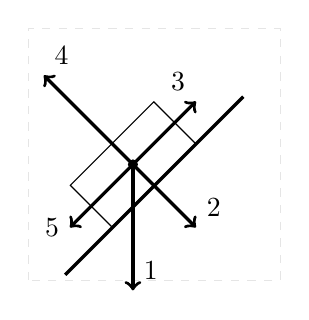
\begin{tikzpicture}[scale=0.8]
                \draw[dashed,white!90!black] (-2,-1.5) rectangle (2,2.5);
                \node[draw,minimum width=1.5cm,minimum height=0.75cm,anchor=south,rotate=45] (B) at (0,0) {};
                \draw[very thick,rotate=45] (-2,0) -- (2,0);
                \draw[fill] (B.center) circle (2pt);
                \draw[very thick,->] (B.center) -- ++(270:2) node[anchor=south west] {1};
                \draw[very thick,->] (B.center) -- ++(315:1.414) node[anchor=south west] {2};
                \draw[very thick,->] (B.center) -- ++(45:1.414) node[anchor=south east] {3};
                \draw[very thick,->] (B.center) -- ++(135:2) node[anchor=south west] {4};
                \draw[very thick,->] (B.center) -- ++(225:1.414) node[anchor=east] {5};
            \end{tikzpicture}
        }
    \end{choices}
    \end{multicols}
\end{question}
}

\element{FBD}{
\begin{question}{FBD-Q06}
    A block is sliding down an inclined plane at constant speed.
    Which of the following diagrams correctly shows the forces acting on the block?
    \begin{multicols}{2}
    \begin{choices}
        \AMCboxDimensions{down=-1.5cm}
        %% B from 5
        \correctchoice{
            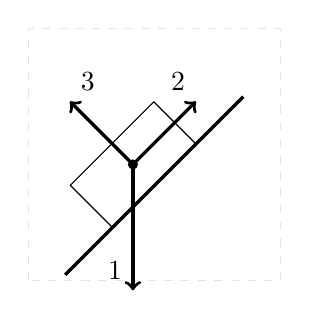
\begin{tikzpicture}[scale=0.8]
                \draw[dashed,white!90!black] (-2,-1.5) rectangle (2,2.5);
                \node[draw,minimum width=1.5cm,minimum height=0.75cm,anchor=south,rotate=45] (B) at (0,0) {};
                \draw[very thick,rotate=45] (-2,0) -- (2,0);
                \draw[fill] (B.center) circle (2pt);
                \draw[very thick,->] (B.center) -- ++(270:2) node[anchor=south east] {1};
                \draw[very thick,->] (B.center) -- ++(45:1.414) node[anchor=south east] {2};
                \draw[very thick,->] (B.center) -- ++(135:1.414) node[anchor=south west] {3};
            \end{tikzpicture}
        }
        %% E from 5
        \wrongchoice{
            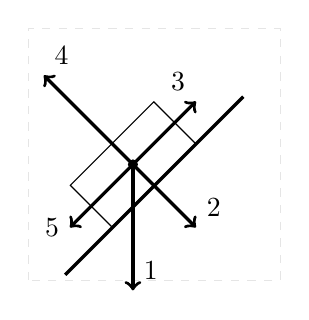
\begin{tikzpicture}[scale=0.8]
                \draw[dashed,white!90!black] (-2,-1.5) rectangle (2,2.5);
                \node[draw,minimum width=1.5cm,minimum height=0.75cm,anchor=south,rotate=45] (B) at (0,0) {};
                \draw[very thick,rotate=45] (-2,0) -- (2,0);
                \draw[fill] (B.center) circle (2pt);
                \draw[very thick,->] (B.center) -- ++(270:2) node[anchor=south west] {1};
                \draw[very thick,->] (B.center) -- ++(315:1.414) node[anchor=south west] {2};
                \draw[very thick,->] (B.center) -- ++(45:1.414) node[anchor=south east] {3};
                \draw[very thick,->] (B.center) -- ++(135:2) node[anchor=south west] {4};
                \draw[very thick,->] (B.center) -- ++(225:1.414) node[anchor=east] {5};
            \end{tikzpicture}
        }
        %% orig
        \wrongchoice{
            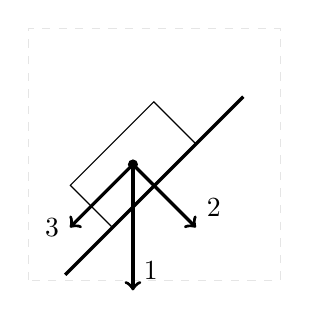
\begin{tikzpicture}[scale=0.8]
                \draw[dashed,white!90!black] (-2,-1.5) rectangle (2,2.5);
                \node[draw,minimum width=1.5cm,minimum height=0.75cm,anchor=south,rotate=45] (B) at (0,0) {};
                \draw[very thick,rotate=45] (-2,0) -- (2,0);
                \draw[fill] (B.center) circle (2pt);
                \draw[very thick,->] (B.center) -- ++(270:2) node[anchor=south west] {1};
                \draw[very thick,->] (B.center) -- ++(315:1.414) node[anchor=south west] {2};
                \draw[very thick,->] (B.center) -- ++(225:1.414) node[anchor=east] {3};
            \end{tikzpicture}
        }
        %% D from 5
        \wrongchoice{
            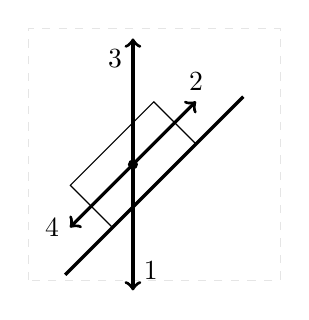
\begin{tikzpicture}[scale=0.8]
                \draw[dashed,white!90!black] (-2,-1.5) rectangle (2,2.5);
                \node[draw,minimum width=1.5cm,minimum height=0.75cm,anchor=south,rotate=45] (B) at (0,0) {};
                \draw[very thick,rotate=45] (-2,0) -- (2,0);
                \draw[fill] (B.center) circle (2pt);
                \draw[very thick,->] (B.center) -- ++(270:2) node[anchor=south west] {1};
                \draw[very thick,->] (B.center) -- ++(45:1.414) node[anchor=south] {2};
                \draw[very thick,->] (B.center) -- ++(90:2) node[anchor=north east] {3};
                \draw[very thick,->] (B.center) -- ++(225:1.414) node[anchor=east] {4};
            \end{tikzpicture}
        }
        %% C from 5
        \wrongchoice{
            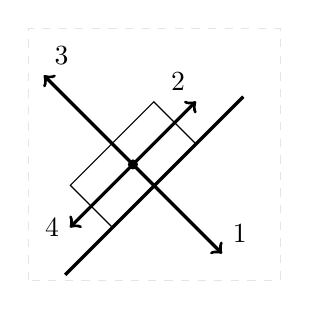
\begin{tikzpicture}[scale=0.8]
                \draw[dashed,white!90!black] (-2,-1.5) rectangle (2,2.5);
                \node[draw,minimum width=1.5cm,minimum height=0.75cm,anchor=south,rotate=45] (B) at (0,0) {};
                \draw[very thick,rotate=45] (-2,0) -- (2,0);
                \draw[fill] (B.center) circle (2pt);
                \draw[very thick,->] (B.center) -- ++(315:2) node[anchor=south west] {1};
                \draw[very thick,->] (B.center) -- ++(45:1.414) node[anchor=south east] {2};
                \draw[very thick,->] (B.center) -- ++(135:2) node[anchor=south west] {3};
                \draw[very thick,->] (B.center) -- ++(225:1.414) node[anchor=east] {4};
            \end{tikzpicture}
        }
    \end{choices}
    \end{multicols}
\end{question}
}

\element{FBD}{
\begin{question}{FBD-Q07}
    A block is sliding down an inclined plane at constant acceleration.
    Which of the following diagrams correctly shows the forces acting on the block?
    \begin{multicols}{2}
    \begin{choices}
        \AMCboxDimensions{down=-1.5cm}
        \wrongchoice{
            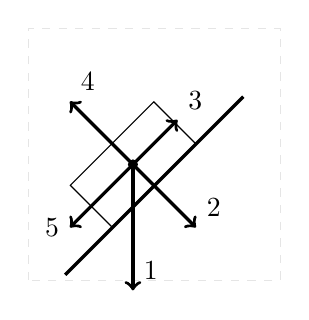
\begin{tikzpicture}[scale=0.8]
                \draw[dashed,white!90!black] (-2,-1.5) rectangle (2,2.5);
                \node[draw,minimum width=1.5cm,minimum height=0.75cm,anchor=south,rotate=45] (B) at (0,0) {};
                \draw[very thick,rotate=45] (-2,0) -- (2,0);
                \draw[fill] (B.center) circle (2pt);
                \draw[very thick,->] (B.center) -- ++(270:2) node[anchor=south west] {1};
                \draw[very thick,->] (B.center) -- ++(315:1.414) node[anchor=south west] {2};
                \draw[very thick,->] (B.center) -- ++(45:1) node[anchor=south west] {3};
                \draw[very thick,->] (B.center) -- ++(135:1.414) node[anchor=south west] {4};
                \draw[very thick,->] (B.center) -- ++(225:1.414) node[anchor=east] {5};
            \end{tikzpicture}
        }
        \correctchoice{
            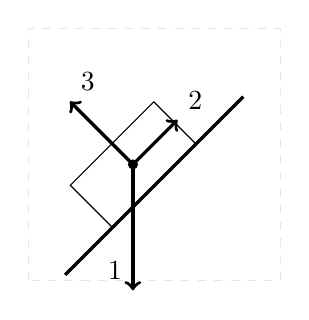
\begin{tikzpicture}[scale=0.8]
                \draw[dashed,white!90!black] (-2,-1.5) rectangle (2,2.5);
                \node[draw,minimum width=1.5cm,minimum height=0.75cm,anchor=south,rotate=45] (B) at (0,0) {};
                \draw[very thick,rotate=45] (-2,0) -- (2,0);
                \draw[fill] (B.center) circle (2pt);
                \draw[very thick,->] (B.center) -- ++(270:2) node[anchor=south east] {1};
                \draw[very thick,->] (B.center) -- ++(45:1) node[anchor=south west] {2};
                \draw[very thick,->] (B.center) -- ++(135:1.414) node[anchor=south west] {3};
            \end{tikzpicture}
        }
        \wrongchoice{
            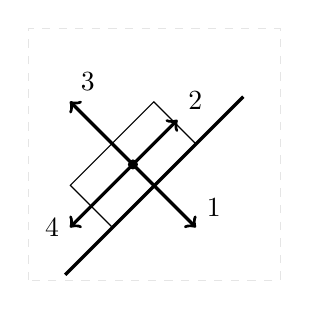
\begin{tikzpicture}[scale=0.8]
                \draw[dashed,white!90!black] (-2,-1.5) rectangle (2,2.5);
                \node[draw,minimum width=1.5cm,minimum height=0.75cm,anchor=south,rotate=45] (B) at (0,0) {};
                \draw[very thick,rotate=45] (-2,0) -- (2,0);
                \draw[fill] (B.center) circle (2pt);
                \draw[very thick,->] (B.center) -- ++(315:1.414) node[anchor=south west] {1};
                \draw[very thick,->] (B.center) -- ++(45:1) node[anchor=south west] {2};
                \draw[very thick,->] (B.center) -- ++(135:1.414) node[anchor=south west] {3};
                \draw[very thick,->] (B.center) -- ++(225:1.414) node[anchor=east] {4};
            \end{tikzpicture}
        }
        \wrongchoice{
            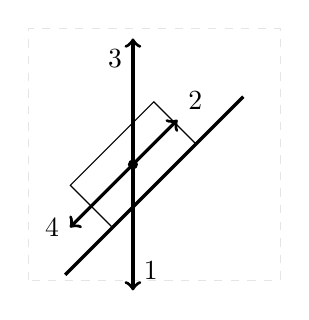
\begin{tikzpicture}[scale=0.8]
                \draw[dashed,white!90!black] (-2,-1.5) rectangle (2,2.5);
                \node[draw,minimum width=1.5cm,minimum height=0.75cm,anchor=south,rotate=45] (B) at (0,0) {};
                \draw[very thick,rotate=45] (-2,0) -- (2,0);
                \draw[fill] (B.center) circle (2pt);
                \draw[very thick,->] (B.center) -- ++(270:2) node[anchor=south west] {1};
                \draw[very thick,->] (B.center) -- ++(45:1) node[anchor=south west] {2};
                \draw[very thick,->] (B.center) -- ++(90:2) node[anchor=north east] {3};
                \draw[very thick,->] (B.center) -- ++(225:1.414) node[anchor=east] {4};
            \end{tikzpicture}
        }
        \wrongchoice{
            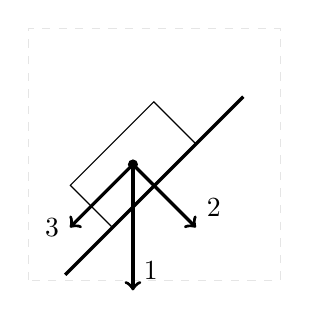
\begin{tikzpicture}[scale=0.8]
                \draw[dashed,white!90!black] (-2,-1.5) rectangle (2,2.5);
                \node[draw,minimum width=1.5cm,minimum height=0.75cm,anchor=south,rotate=45] (B) at (0,0) {};
                \draw[very thick,rotate=45] (-2,0) -- (2,0);
                \draw[fill] (B.center) circle (2pt);
                \draw[very thick,->] (B.center) -- ++(270:2) node[anchor=south west] {1};
                \draw[very thick,->] (B.center) -- ++(315:1.414) node[anchor=south west] {2};
                \draw[very thick,->] (B.center) -- ++(225:1.414) node[anchor=east] {3};
            \end{tikzpicture}
        }
    \end{choices}
    \end{multicols}
\end{question}
}

\element{FBD}{
\begin{question}{FBD-Q08}
    Two men are resting while they are pulling the rope between them.
    \begin{center}
    \begin{tikzpicture}
        %% Ground
        \node[anchor=north,fill,pattern=north east lines,minimum width=6cm, minimum height=0.05cm] at (0,0) {};
        \draw (-3,0) -- (3,0);
        %% Men
        \foreach \x in {-2.5,2.5} {
            \begin{scope}[anchor=south,xshift=\x cm,scale=2.0]
                \draw[thick] (0,0.25) -- (0,0.75);
                %% Legs
                \draw[thick] (0,0.25) -- (-0.25,0);
                \draw[thick] (0,0.25) -- (+0.25,0);
                %% Arms
                \draw[thick] (0,0.50) -- (-0.25,0.55);
                \draw[thick] (0,0.50) -- (+0.25,0.55);
                %% Head
                \draw[fill=white!90!black] (0,0.80) circle (0.15cm);
            \end{scope}
        }
        %% Rope
        \draw[very thick,<->] (-2,1.1) -- (2,1.1);
    \end{tikzpicture}
    \end{center}
    Which of the following diagrams correctly shows the forces acting on the left man?
    \begin{multicols}{2}
    \begin{choices}
        \AMCboxDimensions{down=-1.5cm}
        \correctchoice{
            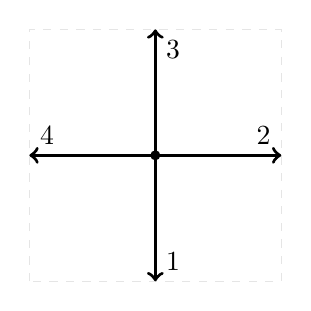
\begin{tikzpicture}[scale=0.8]
                \draw[dashed,white!90!black] (-2,-2) rectangle (2,2);
                \coordinate (B) at (0,0);
                \draw[fill] (B) circle (2pt);
                \draw[very thick,->] (B) -- ++(270:2) node[anchor=south west] {1};
                \draw[very thick,->] (B) -- ++(0:2) node[anchor=south east] {2};
                \draw[very thick,->] (B) -- ++(90:2) node[anchor=north west] {3};
                \draw[very thick,->] (B) -- ++(180:2) node[anchor=south west] {4};
            \end{tikzpicture}
        }
        \wrongchoice{
            \begin{tikzpicture}[scale=0.8]
                \draw[dashed,white!90!black] (-2,-2) rectangle (2,2);
                \coordinate (B) at (0,0);
                \draw[fill] (B) circle (2pt);
                \draw[very thick,->] (B) -- ++(0:2) node[anchor=south east] {1};
                \draw[very thick,->] (B) -- ++(180:2) node[anchor=south west] {2};
            \end{tikzpicture}
        }
        \wrongchoice{
            \begin{tikzpicture}[scale=0.8]
                \draw[dashed,white!90!black] (-2,-2) rectangle (2,2);
                \coordinate (B) at (0,0);
                \draw[fill] (B) circle (2pt);
                \draw[very thick,->] (B) -- ++(0:2) node[anchor=south east] {1};
            \end{tikzpicture}
        }
        \wrongchoice{
            \begin{tikzpicture}[scale=0.8]
                \draw[dashed,white!90!black] (-2,-2) rectangle (2,2);
                \coordinate (B) at (0,0);
                \draw[fill] (B) circle (2pt);
                \draw[very thick,->] (B) -- ++(270:2) node[anchor=south west] {1};
                \draw[very thick,->] (B) -- ++(0:2) node[anchor=south east] {2};
            \end{tikzpicture}
        }
        \wrongchoice{
            \begin{tikzpicture}[scale=0.8]
                \draw[dashed,white!90!black] (-2,-2) rectangle (2,2);
                \coordinate (B) at (0,0);
                \draw[fill] (B) circle (2pt);
                \draw[very thick,->] (B) -- ++(270:2) node[anchor=south west] {1};
                \draw[very thick,->] (B) -- ++(90:2) node[anchor=north west] {2};
            \end{tikzpicture}
        }
    \end{choices}
    \end{multicols}
\end{question}
}

\element{FBD}{
\begin{question}{FBD-Q09}
    Two men are resting while they are pulling the rope between them.
    In doing so, the stronger man (on the right side of the rope) is at rest,
        and the weaker man (on the left side of the rope) is sliding to the right.
    \begin{center}
    \begin{tikzpicture}
        %% Ground
        \node[anchor=north,fill,pattern=north east lines,minimum width=6cm, minimum height=0.05cm] at (0,0) {};
        \draw (-3,0) -- (3,0);
        %% Men
        \foreach \x in {-2.5,2.5} {
            \begin{scope}[anchor=south,xshift=\x cm,scale=2.0]
                \draw[thick] (0,0.25) -- (0,0.75);
                %% Legs
                \draw[thick] (0,0.25) -- (-0.25,0);
                \draw[thick] (0,0.25) -- (+0.25,0);
                %% Arms
                \draw[thick] (0,0.50) -- (-0.25,0.55);
                \draw[thick] (0,0.50) -- (+0.25,0.55);
                %% Head
                \draw[fill=white!90!black] (0,0.80) circle (0.15cm);
            \end{scope}
        }
        %% Rope
        \draw[very thick,<->] (-2,1.1) -- (2,1.1);
    \end{tikzpicture}
    \end{center}
    Which of the following diagrams correctly shows the forces acting on the left man when his motion starts?
    \begin{multicols}{2}
    \begin{choices}
        \AMCboxDimensions{down=-1.5cm}
        \wrongchoice{
            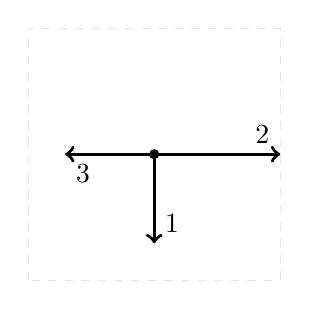
\begin{tikzpicture}[scale=0.8]
                \draw[dashed,white!90!black] (-2,-2) rectangle (2,2);
                \coordinate (B) at (0,0);
                \draw[fill] (B) circle (2pt);
                \draw[very thick,->] (B) -- ++(270:1.414) node[anchor=south west] {1};
                \draw[very thick,->] (B) -- ++(0:2) node[anchor=south east] {2};
                \draw[very thick,->] (B) -- ++(180:1.414) node[anchor=north west] {3};
            \end{tikzpicture}
        }
        \wrongchoice{
            \begin{tikzpicture}[scale=0.8]
                \draw[dashed,white!90!black] (-2,-2) rectangle (2,2);
                \coordinate (B) at (0,0);
                \draw[fill] (B) circle (2pt);
                \draw[very thick,->] (B) -- ++(270:2) node[anchor=south west] {1};
                \draw[very thick,->] (B) -- ++(0:2) node[anchor=south east] {2};
            \end{tikzpicture}
        }
        \wrongchoice{
            \begin{tikzpicture}[scale=0.8]
                \draw[dashed,white!90!black] (-2,-2) rectangle (2,2);
                \coordinate (B) at (0,0);
                \draw[fill] (B) circle (2pt);
                \draw[very thick,->] (B) -- ++(0:2) node[anchor=south east] {1};
                \draw[very thick,->] (B) -- ++(180:1.414) node[anchor=south west] {2};
            \end{tikzpicture}
        }
        \wrongchoice{
            \begin{tikzpicture}[scale=0.8]
                \draw[dashed,white!90!black] (-2,-2) rectangle (2,2);
                \coordinate (B) at (0,0);
                \draw[fill] (B) circle (2pt);
                \draw[very thick,->] (B) -- ++(0:2) node[anchor=south east] {1};
            \end{tikzpicture}
        }
        \correctchoice{
            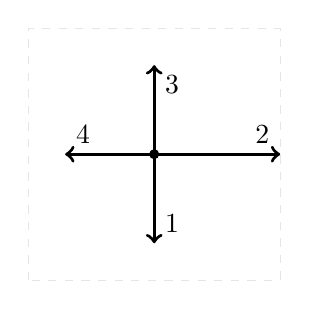
\begin{tikzpicture}[scale=0.8]
                \draw[dashed,white!90!black] (-2,-2) rectangle (2,2);
                \coordinate (B) at (0,0);
                \draw[fill] (B) circle (2pt);
                \draw[very thick,->] (B) -- ++(270:1.414) node[anchor=south west] {1};
                \draw[very thick,->] (B) -- ++(0:2) node[anchor=south east] {2};
                \draw[very thick,->] (B) -- ++(90:1.414) node[anchor=north west] {3};
                \draw[very thick,->] (B) -- ++(180:1.414) node[anchor=south west] {4};
            \end{tikzpicture}
        }
    \end{choices}
    \end{multicols}
\end{question}
}

\element{FBD}{
\begin{question}{FBD-Q10}
    The pendulum bob is swinging from right to left,
        starting from a position higher than the one shown in figure.
    If we neglect air resistance,
        which of the following diagrams correctly shows the forces acting on the pendulum bob?
    \begin{multicols}{2}
    \begin{choices}
        \AMCboxDimensions{down=-1.5cm}
        \wrongchoice{
            \begin{tikzpicture}[scale=1.0]
                \draw[dashed,white!90!black] (-0.6,0.3) rectangle (2.5,-4);
                %% Ceiling
                \node[anchor=south,fill,pattern=north east lines,minimum width=1cm, minimum height=0.05cm] at (0,0) {};
                \draw (-0.5,0) -- (0.5,0);
                %% pendulum
                \coordinate (P) at (300:2.5cm);
                \draw[thick,fill=white!90!black] (P) circle (0.2cm);
                \draw[fill] (P) circle (1pt);
                \draw (0,0) -- (P);
                %% vectors
                \draw[very thick,->] (P) -- ++(120:1) node[anchor=south west] {4};
                \draw[very thick,->] (P) -- ++(30:0.707) node[anchor=south east] {3};
                \draw[very thick,->] (P) -- ++(210:0.707) node[anchor=south east] {5};
                \draw[very thick,->] (P) -- ++(270:1.414) node[anchor=south west] {1};
                \draw[very thick,->] (P) -- ++(300:1.225) node[anchor=south west] {2};
            \end{tikzpicture}
        }
        \correctchoice{
            \begin{tikzpicture}[scale=1.0]
                \draw[dashed,white!90!black] (-0.6,0.3) rectangle (2.5,-4);
                %% Ceiling
                \node[anchor=south,fill,pattern=north east lines,minimum width=1cm, minimum height=0.05cm] at (0,0) {};
                \draw (-0.5,0) -- (0.5,0);
                %% pendulum
                \coordinate (P) at (300:2.5cm);
                \draw[thick,fill=white!90!black] (P) circle (0.2cm);
                \draw[fill] (P) circle (1pt);
                \draw (0,0) -- (P);
                %% vectors
                \draw[very thick,->] (P) -- ++(120:1) node[anchor=south west] {2};
                \draw[very thick,->] (P) -- ++(270:1.414) node[anchor=south west] {1};
            \end{tikzpicture}
        }
        \wrongchoice{
            \begin{tikzpicture}[scale=1.0]
                \draw[dashed,white!90!black] (-0.6,0.3) rectangle (2.5,-4);
                %% Ceiling
                \node[anchor=south,fill,pattern=north east lines,minimum width=1cm, minimum height=0.05cm] at (0,0) {};
                \draw (-0.5,0) -- (0.5,0);
                %% pendulum
                \coordinate (P) at (300:2.5cm);
                \draw[thick,fill=white!90!black] (P) circle (0.2cm);
                \draw[fill] (P) circle (1pt);
                \draw (0,0) -- (P);
                %% vectors
                \draw[very thick,->] (P) -- ++(120:1) node[anchor=south west] {2};
                \draw[very thick,->] (P) -- ++(270:1.414) node[anchor=south west] {1};
                \draw[very thick,->] (P) -- ++(210:0.707) node[anchor=south] {3};
            \end{tikzpicture}
        }
        \wrongchoice{
            \begin{tikzpicture}[scale=1.0]
                \draw[dashed,white!90!black] (-0.6,0.3) rectangle (2.5,-4);
                %% Ceiling
                \node[anchor=south,fill,pattern=north east lines,minimum width=1cm, minimum height=0.05cm] at (0,0) {};
                \draw (-0.5,0) -- (0.5,0);
                %% pendulum
                \coordinate (P) at (300:2.5cm);
                \draw[thick,fill=white!90!black] (P) circle (0.2cm);
                \draw[fill] (P) circle (1pt);
                \draw (0,0) -- (P);
                %% vectors
                \draw[very thick,->] (P) -- ++(270:1.414) node[anchor=south west] {1};
                \draw[very thick,->] (P) -- ++(300:1.225) node[anchor=south west] {2};
                \draw[very thick,->] (P) -- ++(120:1.225) node[anchor=south west] {3};
                \draw[very thick,->] (P) -- ++(210:0.707) node[anchor=south east] {4};
            \end{tikzpicture}
        }
        \wrongchoice{
            \begin{tikzpicture}[scale=1.0]
                \draw[dashed,white!90!black] (-0.6,0.3) rectangle (2.5,-4);
                %% Ceiling
                \node[anchor=south,fill,pattern=north east lines,minimum width=1cm, minimum height=0.05cm] at (0,0) {};
                \draw (-0.5,0) -- (0.5,0);
                %% pendulum
                \coordinate (P) at (300:2.5cm);
                \draw[thick,fill=white!90!black] (P) circle (0.2cm);
                \draw[fill] (P) circle (1pt);
                \draw (0,0) -- (P);
                %% vectors
                \draw[very thick,->] (P) -- ++(210:1) node[anchor=south] {1};
            \end{tikzpicture}
        }
    \end{choices}
    \end{multicols}
\end{question}
}

\element{FBD}{
\begin{question}{FBD-Q11}
    The ball is in circular clockwise motion along a horizontal channel.
    If we neglect friction and air resistance,
        which of the following diagrams correctly shows the forces acting on the ball?
    \begin{multicols}{2}
    \begin{choices}
        \AMCboxDimensions{down=-1cm}
        \wrongchoice{
            \begin{tikzpicture}[scale=0.7]
                \draw (0,0) circle (2cm and 0.55cm);
                \draw (0,0) circle (2.2cm and 0.6cm);
                \coordinate (B) at (-1,-0.5);
                \draw[fill,rotate=-10] (B) circle (4pt and 3pt);
                \draw[thick,->] (B) -- ++(270:1.414) node[anchor=south west] {1};
                \draw[thick,->] (B) -- ++(90:1.414) node[anchor=north west] {2};
                \draw[thick,->] (B) -- ++(-1.2,0.3) node[anchor=north west] {3};
            \end{tikzpicture}
        }
        \wrongchoice{
            \begin{tikzpicture}[scale=0.7]
                \draw (0,0) circle (2cm and 0.55cm);
                \draw (0,0) circle (2.2cm and 0.6cm);
                \coordinate (B) at (-1,-0.5);
                \draw[fill,rotate=-10] (B) circle (4pt and 3pt);
                \draw[thick,->] (B) -- ++(270:1.414) node[anchor=south west] {1};
                \draw[thick,->] (B) -- ++(90:1.414) node[anchor=north west] {2};
                \draw[thick,->] (B) -- ++(-1,-0.5) node[anchor=north west] {3};
            \end{tikzpicture}
        }
        \correctchoice{
            \begin{tikzpicture}[scale=0.7]
                \draw (0,0) circle (2cm and 0.55cm);
                \draw (0,0) circle (2.2cm and 0.6cm);
                \coordinate (B) at (-1,-0.5);
                \draw[fill,rotate=-10] (B) circle (4pt and 3pt);
                \draw[thick,->] (B) -- ++(270:1.414) node[anchor=south west] {1};
                \draw[thick,->] (B) -- ++(1,0.5) node[anchor=west] {2};
                \draw[thick,->] (B) -- ++(90:1.414) node[anchor=north west] {3};
            \end{tikzpicture}
        }
        \wrongchoice{
            \begin{tikzpicture}[scale=0.7]
                \draw (0,0) circle (2cm and 0.55cm);
                \draw (0,0) circle (2.2cm and 0.6cm);
                \coordinate (B) at (-1,-0.5);
                \draw[fill,rotate=-10] (B) circle (4pt and 3pt);
                \draw[thick,->] (B) -- ++(270:1.414) node[anchor=south west] {1};
                \draw[thick,->] (B) -- ++(90:1.414) node[anchor=north west] {3};
                \draw[thick,->] (B) -- ++(1,0.5) node[anchor=west] {2};
                \draw[thick,->] (B) -- ++(-1,-0.5) node[anchor=north west] {4};
            \end{tikzpicture}
        }
        \wrongchoice{
            \begin{tikzpicture}[scale=0.7]
                \draw (0,0) circle (2cm and 0.55cm);
                \draw (0,0) circle (2.2cm and 0.6cm);
                \coordinate (B) at (-1,-0.5);
                \draw[fill,rotate=-10] (B) circle (4pt and 3pt);
                \draw[thick,->] (B) -- ++(270:1.414) node[anchor=south west] {1};
                \draw[thick,->] (B) -- ++(1,0.5) node[anchor=west] {2};
            \end{tikzpicture}
        }
    \end{choices}
    \end{multicols}
\end{question}
}

\element{FBD}{
\begin{question}{FBD-Q12}
    The ball is in a clockwise motion along a verical circular loop.
    If we neglect friction and air resistance,
        which of the following diagrams correctly shows the forces acting on the ball?
    \begin{multicols}{2}
    \begin{choices}
        \AMCboxDimensions{down=-2cm}
        \wrongchoice{
            \begin{tikzpicture}[scale=0.75]
                \draw[thick] (0,0) circle (2cm);
                \coordinate (B) at (0,-1.8cm);
                \draw[thick,fill=white!90!black] (B) circle (0.2cm);
                \draw[fill] (B) circle (1pt);
                \draw[thick,->] (B) -- ++(180:1.414) node[anchor=north west] {2};
                \draw[thick,->] (B) -- ++(270:1.414) node[anchor=south west] {1};
            \end{tikzpicture}
        }
        \wrongchoice{
            \begin{tikzpicture}[scale=0.75]
                \draw[thick] (0,0) circle (2cm);
                \coordinate (B) at (0,-1.8cm);
                \draw[thick,fill=white!90!black] (B) circle (0.2cm);
                \draw[fill] (B) circle (1pt);
                \draw[thick,->] (B) -- ++(90:0.707) node[anchor=west] {2};
                \draw[thick,->] (B) -- ++(270:1.414) node[anchor=south west] {1};
            \end{tikzpicture}
        }
        \correctchoice{
            \begin{tikzpicture}[scale=0.75]
                \draw[thick] (0,0) circle (2cm);
                \coordinate (B) at (0,-1.8cm);
                \draw[thick,fill=white!90!black] (B) circle (0.2cm);
                \draw[fill] (B) circle (1pt);
                \draw[thick,->] (B) -- ++(90:2.8) node[anchor=north west] {2};
                \draw[thick,->] (B) -- ++(270:1.414) node[anchor=south west] {1};
            \end{tikzpicture}
        }
        \wrongchoice{
            \begin{tikzpicture}[scale=0.75]
                \draw[thick] (0,0) circle (2cm);
                \coordinate (B) at (0,-1.8cm);
                \draw[thick,fill=white!90!black] (B) circle (0.2cm);
                \draw[fill] (B) circle (1pt);
                \draw[thick,->] (B) -- ++(90:1.414) node[anchor=north west] {2};
                \draw[thick,->] (B) -- ++(270:1.414) node[anchor=south west] {1};
            \end{tikzpicture}
        }
        \wrongchoice{
            \begin{tikzpicture}[scale=0.75]
                \draw[thick] (0,0) circle (2cm);
                \coordinate (B) at (0,-1.8cm);
                \draw[thick,fill=white!90!black] (B) circle (0.2cm);
                \draw[fill] (B) circle (1pt);
                \draw[thick,->] (B) -- ++(90:1.414) node[anchor=north west] {2};
                \draw[thick,->] (B) -- ++(270:1.414) node[anchor=south west] {1};
                \draw[thick,->] (B) -- ++(180:1.414) node[anchor=north west] {3};
            \end{tikzpicture}
        }
    \end{choices}
    \end{multicols}
\end{question}
}


\endinput


